\documentclass{article}
\usepackage{amsmath,amssymb,amsthm, graphicx, float, subfig}
\usepackage{mathpazo}
\author{Alexandre Vassalotti \quad \'{E}ric Renaud-Houde}
\title{COMP 558: Final Project Report \\
  \large \textbf{Surface reconstruction using the level set method}
}
\date{27 April 2012}
\setcounter{secnumdepth}{3}
\begin{document}
\maketitle
\section{Introduction}
Modelling surfaces from unorganized set of points, or point clouds, is a long
standing problem in the computer vision community. Indeed, problem is known to
be very challenging in three and higher dimensions. Furthermore, the problem
is ill-posed which means there is not a unique solution. When the point cloud
is dense enough and the topology of the surface is not complicated, a simple
solution could be to perform a Denaulay triangulation of points, as
described by Boissonnat \cite{boissonnat1984geometric}. However, even in this
context ambiguities can arises and lead to non desirable surface
reconstructions.

A desirable reconstruction method should be able to deal with irregularities
caused by noise and non-uniformity of the data collected. It should also be
able to deal with complex surface topologies as well. In addition, the
reconstructed surface should be representative of the point cloud. It should
be reasonably smooth yet maintain discontinuities.

Many approaches have been proposed to solve the surface reconstruction
problem. In general, the solutions can be categorized by the surface
representation they use---i.e, explicit or implicit. In an explicit
representation, the location of all the points on the surface is described
precisely. Triangulations methods yield such representations. Conversely, in
an implicit representation, we describe the surface as a constraint in a
higher dimension, or 3D space in our case. Implicit representations are often
advantageous because they lead to solutions capablable of handling complex
topologies. Their main drawback is they tend to be more expensive in time and
space.

level set methods are a class of techniques for the deformation of implicit
surfaces according to arbitrary rules. These methods were developed conjointly
by Osher and Sethian \cite{sethian1999level} and are widely applicable to a
variety of problems. In the context of surface reconstruction, Zhao showed
\cite{zhao2001fast} how to apply these methods to minimize a given energy
functional which is analogous to a least-square fitting on a point cloud. This
is the approach we will explore in this report.

Our final project was motivated by the arrival of low-cost depth sensors, such
as the Microsoft's Kinect. The opportunities for object and scene
reconstruction using these sensors are obvious. These depth sensors provide
accurate and dense measurements. A caveat however is these new devices are
typically structured light sensors. And the data from such devices have large
holes due to the shadows casted by the objects being measured. This poses
extras challenges for surfaces reconstruction.

\begin{figure}
  \centering
  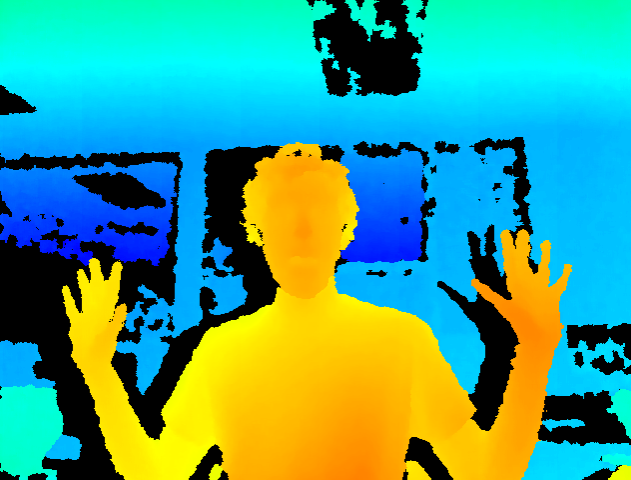
\includegraphics[width=0.7\textwidth]{img/depthmap.png}
  \caption{In this depth image taken using Microsoft's Kinect sensor, we see
holes, represented as black regions, where the sensor couldn't take
measurements.}

\end{figure}

\section{Level set method}
The level set method involves the evolution of a function, called $\phi$,
using an iterative scheme for numerical integration. The surface we wish to
recover is represented as a constraint on $\phi$. Specifically, we define this
surface as the level set $\Gamma=\{\mathbf{x}:\phi(\mathbf{x}, t)=0\}$.

The central problem of the level set method is to propagate the surface
$\Gamma$ like a firefront. If a velocity field $\vec{v}$ gives the direction
and speed of each point for movement, then the evolution of the surface
$\Gamma$ over time $t$ is described by the equation

\begin{align}
  \frac{d \Gamma}{dt} = \vec{v}
\end{align}

This can be reformulated for $\phi$ to yield the fundamental level set
equation
\begin{align}
  \frac{d \phi}{dt} + \vec{v} \cdot \nabla \phi = 0
\end{align}

We have yet to define the level set function $\phi$. One particularly
attractive definition is the signed distance function $d(\mathbf{x})$, which
gives the distance of a point to the surface and the sign: generally $d > 0$
if the point $\mathbf{x}$ is outside and $d < 0$ if it is inside of the
surface (assuming it is a closed surface). Although all definitions of $\phi$
are equally good theoretically, we prefer the signed distance function to
avoid numerical instabilities and inaccuracies during computations. But even
with this definition, $\phi$ will not remain a signed distance function and we
may need a reinitialization procedure to keep the level set intact
\cite{peng1999pde}.

Another advantage of the signed distance function is the fact that the
gradient $\nabla d(\mathbf{x})$ is a unit vector for all
$\mathbf{x}$. Moreover, it is the unit normal $\vec{n}(\mathbf{x})$ to the
level sets.

\subsection{Discretization}

Given that the surface motion equation for $\phi$ is defined as a partial
differential equation, we can solve it using iterative schemes for PDEs. As most
differential equations which might appear fairly innocuous at first, solving
them numerically can be quite challenging.

Given an initial value $\phi_0$, our first intution might be to apply the
first-order Euler method as follows:
\begin{align}
  \frac{\partial \phi}{\partial t} + F \|\nabla \phi\| &= 0 \\
  \frac{\phi^{t+1} - \phi^{t}}{\Delta t} &=  -F \|\nabla \phi\| \\
  \phi^{t+1} &= \phi^{t} - \Delta t \; F \|\nabla \phi\| 
\end{align}

However, not only does the Euler method often suffers from stability problems,
it is used in the context of \textit{ordinary differential equations}, not PDEs.
In that case, a different numerical procedure is needed. 

\subsubsection{Upwind Scheme}
One approach for discretizing PDEs, originally defined by Couran, Isaacson and
Rees \cite{courant1952solution} is called the upwind scheme. Instead of using
central differences for computing the partial derivatives, it uses both a
forward or a backward difference:

\begin{align}
    \frac{\partial p}{\partial x}^{-} &= p^{-}_x = \frac{p_i -
    p_{i-1}}{ \Delta x} = p_i - p_{i-1} \\
    \frac{\partial p}{\partial x}^{+} &= p^{+}_x = \frac{p^{i+1}_x -
    p^i_x}{ \Delta x} = p^{i+1}_x - p^i_x  
\end{align} since $ \Delta x = 1 $ in our grid. The same applies for other axes
$y$ and $z$.

\begin{figure}[htb]
  \centering
  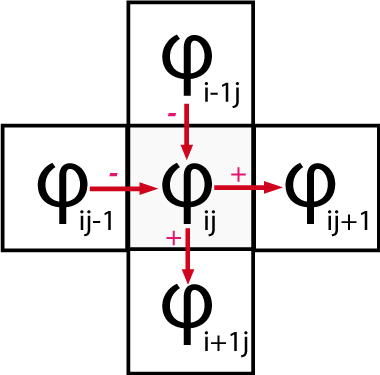
\includegraphics[width=0.45\textwidth]{img/upwind_grid.png}
  \caption{Illustration of the forward and backward differences over a 2d grid.}    
\end{figure}


Later used by Sethian\cite{sethian1999level} \cite{sethian1999advancing} for the
initial value formulation, he defines the (now standard) level set method as
follows (let $ p = \phi_{ijk}$):

\[
p^{n+1} = p^{n} - \Delta t [ \max(F_{ijk}, 0) \| \nabla p \|^{+} + \min(F_{ijk},
0) \| \nabla p \|^{-} ]
\]
where:
\begin{align}
    \| \nabla p \|^{+} & = 
    \begin{bmatrix}
        \max(p^{-}_x, 0)^2 + \min(p^{+}_x, 0)^2 + \\
        \max(p^{-}_y, 0)^2 + \min(p^{+}_y, 0)^2 + \\
        \max(p^{-}_z, 0)^2 + \min(p^{+}_z, 0)^2
    \end{bmatrix}^{1/2}  \\
    \| \nabla p \|^{-} & = 
    \begin{bmatrix}
        \max(p^{+}_x, 0)^2 + \min(p^{-}_x, 0)^2 + \\
        \max(p^{+}_y, 0)^2 + \min(p^{-}_y, 0)^2 + \\
        \max(p^{+}_z, 0)^2 + \min(p^{-}_z, 0)^2
    \end{bmatrix}^{1/2} 
\end{align}

Rewriting this equation in terms of the entire grid matrices, and defining
$\odot$ as element-wise matrix mutiplication, we have the following formulation
which updates our entire grid for $\phi$:
\[
\phi^{n+1} = \phi^{n} - \Delta t [ \max(F, 0) \odot \| \nabla \phi \|^{+} +
\min(F, 0) \odot \| \nabla \phi \|^{-} ]
\]

As opposed to computing the magnitude of the gradient using the central
differences functions, the evolution of $\phi$ under the upwind scheme is much
more stable. Note that there are higher-order schemes listed in
\cite{sethian1999level} if more stability is required.

\begin{figure}[H]
  \centering
  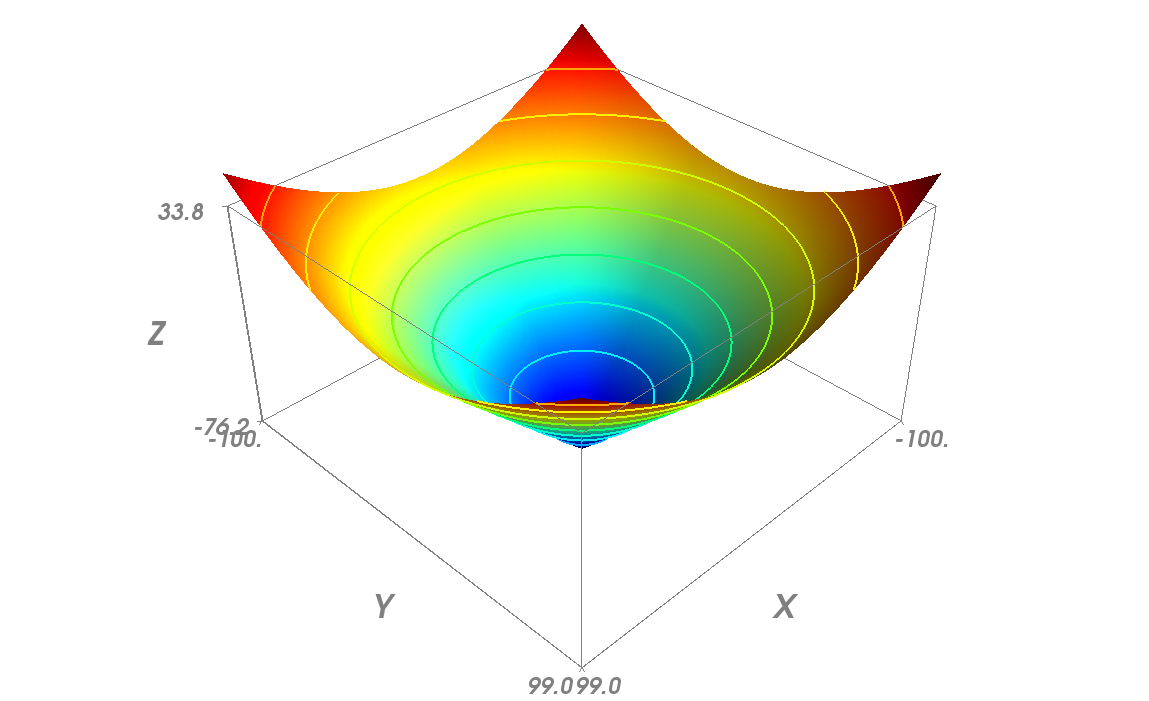
\includegraphics[width=0.8\textwidth]{img/up01.png}
  \caption{Initial hypersurface $\phi$ defined as a signed distance function
  (for a level set in 2d).}    
\end{figure}

\begin{figure}[H]
  \centering
  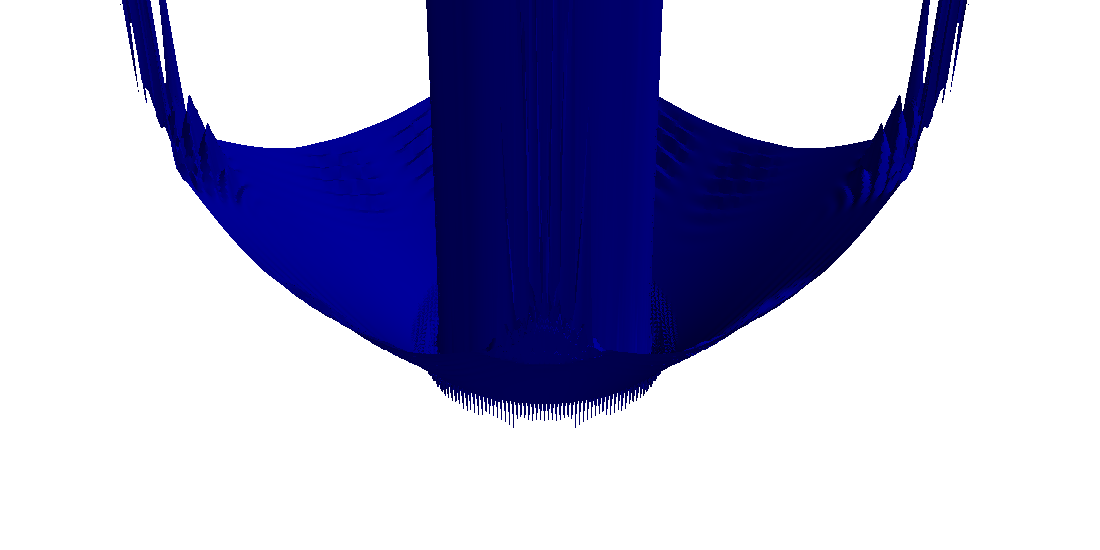
\includegraphics[width=0.8\textwidth]{img/up03.png}
  \caption{Result of 140 iterations using $\Delta t = 0.5$ and a constant force
  of 1 using the central differences approximations. The resulting hypersurface
  has exploded in the center and near the borders.}    
\end{figure}

\begin{figure}[H]
  \centering
  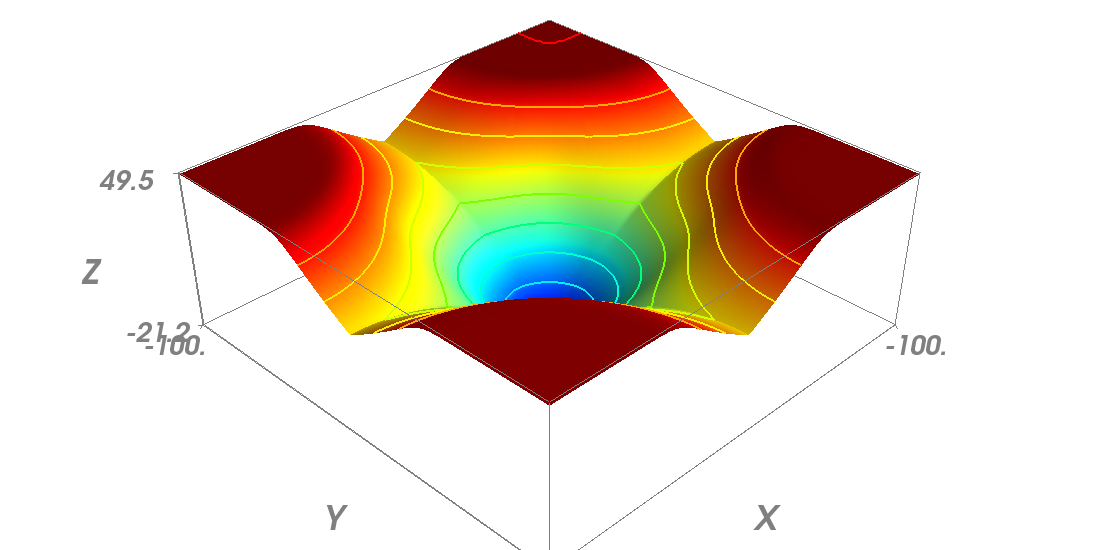
\includegraphics[width=0.8\textwidth]{img/up02.png}
  \caption{Result of 140 iterations using $ \Delta t = 0.5$ and a constant force
  of 1 using the upwind scheme. The hypersurface evolution is perfectly stable.
  It ultimately flattens out and remains so.}    
\end{figure}

\paragraph{Implementation}
To implement the upwind scheme for the entire grid
update, a few strategies can be used. In the contex of matlab or numpy, it is
recommended to compute forward and backward differences using entire rows at
once. Also note that only one matrix is needed to store the results because the
squared differences can be added on top of each other.  Furthermore for the
edges of the grid, the inward row/column should be used in replacement if the
difference exceeds the matrix.

\subsubsection{Adaptive step size}
Based on the work on level set stability and convergence by \textit{Chaudhury
and Ramakrishnan} in \cite{chaudhury2007stability}, an adaptive step size can be
easily implemented to make the evolution as fast as possible. Simply stated, the
stability condition for the level set evolution is:
\[
F_{max} \cdot \Delta t \le \min(\Delta \mathbf{x})
\]
where $F_{max}$ is the maximum absolute speed of all the points on the grid and
$\Delta \mathbf{x}$ is the grid spacing. Since we consider the grid size to be
1, we can adaptively set the step size to the following:
\[
\Delta t \leftarrow q \cdot \frac{1}{F_{max}}
\]
where $q$ is a safety factor (it has a value slightly smaller than 1).



\subsection{Forces governing surface evolution}

Up until now, we have left one variable undefined, namely the force matrix $F$.
The definition of this term very much depends on the application of the
algorithm. For example, a popular approach used in 2d segmentation (for example

in the context of medical imagery) is to employ (the magnitude of)
gradients of the image to limit the evolution of the level set.
However with a point cloud, the force must be derived differently. A
formulation was specifically developped by Zhao in
\cite{zhao2000implicit} and \cite{zhao2001fast} for shape
reconstruction from an unorganized dataset of points. 

Stating his formulation upfront, we have:
\begin{align}
    \label{eq:force}
    F = \nabla d(\mathbf{x}) \cdot \frac{\nabla \phi}{\| \nabla \phi \|}
+ d(\mathbf{x}) \cdot (\nabla \cdot \frac{\nabla \phi}{\| \nabla \phi \|} )
\end{align}
where $d(\mathbf{x})$ is an unsigned distance function to the closest point in
our dataset $S$.

The role of this force is twofold: it simultaneously encourages smoothness in
the level set and close fit to the data points which are attracting it.

\subsubsection{Energy Functional}
To understand where this force formulation comes from, we have to understand how
the desired level set surface is derived from an energy functional $E(\Gamma)$.
Without restating all the derivations, the functional essentially takes in the
level set as its input and assesses its surface energy in terms of distance to
$S$. More precisely, Zhao\cite{zhao2000implicit} defined it as follows:

\begin{align}
    \label{eq:functional}
    E(\Gamma) = [\int_\Gamma d^p(\mathbf{x}) ds]^{1/p}
\end{align}

where $ds$ is the surface area, and $p$ parametrizes the distance (or norm)
function. For the level set to evolve to a local minimum of this energy
functional, it has to flow according to a force which employs not only
$d(\mathbf{x})$ but also the normal $\mathbf{N}$ to $\Gamma$ and the mean
curvature $\kappa$ of $\Gamma$. In fact, in can be shown that the minimizer of
\eqref{eq:functional} satisfies:
\[
\nabla d(\mathbf{x}) \cdot \mathbf{n} + d(\mathbf{x}) \kappa = 0
\]
With these terms used in the force formulation, and with the evolution equation
expressed for $\phi$, equation \eqref{eq:force} is obtained. (See \cite{zhao2000implicit},
\cite{zhao2001fast} and \cite{savadjiev2003surface} for more detailed
explanations.) The resulting level set evolution should then behave as an
elastic membrane converging towards a minimal surface.

%\item Quantifies how $\Gamma$ corresponds to the data set, with a smoothness constraint
%\item Has two global minima: $\Gamma = \Gamma_0$  and $\Gamma = \emptyset$.

\subsubsection{Unsatisfactory local minimum}
\label{localmin}
Note that the level set can reach an unsatisfactory local minimum if the initial
value was not close enough to the final surface. As such, it is expected that
this methods results in some loss of details.

\begin{figure}[H]
  \centering
  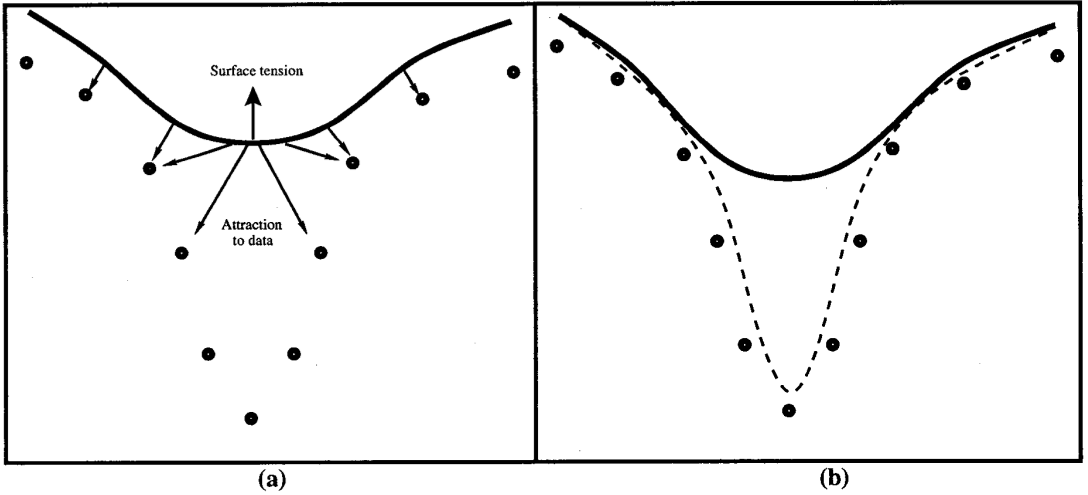
\includegraphics[width=1.0\textwidth]{img/savadjiev3_3.png}
  \caption{This figure taken from \cite{savadjiev2003surface} illustrates
  how the level set might be unable to reach the bottom of a crevasse. The local
  minumum (b) is reached from (a). The surface tension prevents the curve from
  bending and lower points cannot attract the surface further down because they
  are not the closest.}    
\end{figure}

\subsection{Source of errors}
As stated earlier, numerical solutions for solving the level set equation can
very easily become unstable.
\begin{itemize}
    \item \textbf{Reinitialization}: If reinitialization is used, the interface
        can be displaced to incoherent positions, affecting numerical accuracy
        in an undesirable way. This is why it is normally avoided as much as
        possible. Methods have been developped to avoid the need for
        reinitialization entirely, such as \cite{li2010distance} by \emph{Li,
        Xu, Gui and Fox}.
    \item \textbf{Incorrect gradient}: As stated earlier, central differences
        should be avoided.
    \item \textbf{Order of approximation}: First order approximations can lead
        to numerical diffusion, higher order methods are prefered.
    \item \textbf{Force (or speed) function}: The force function might be
        well-defined around the level set but has no guarantees of stability
        further out. This is why a force extension strategy can be used. 
\end{itemize}

\section{Results}
In order to implement of the level set evolution as described above, we first
favored a 2d version implementation in Python (using NumPy, SciPy, Scikit-fmm
(for solving the Eikonal equation) and Matplotlib. Here are our final 2d
results.
\begin{figure}[H]
  \centering
  \subfloat[Initial data set of
  points.]{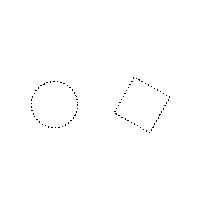
\includegraphics[width=0.50\textwidth]{img/dataset.png}}
  ~
  \subfloat[Unsigned distance function to the data set of
  points.]{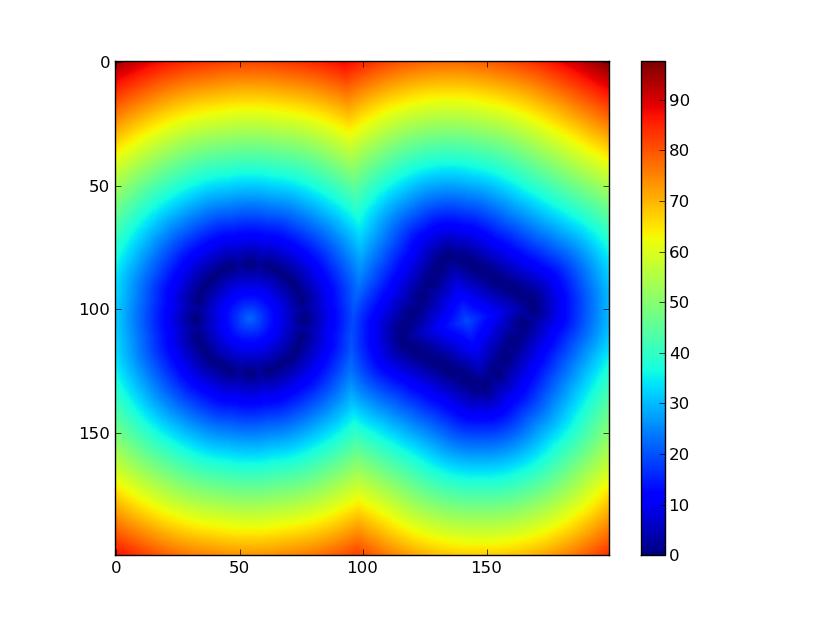
\includegraphics[width=0.50\textwidth]{img/signed_dist.png}} \\
  \subfloat[Initial $\phi$ with the embedded level set curve
  $\Gamma$.]{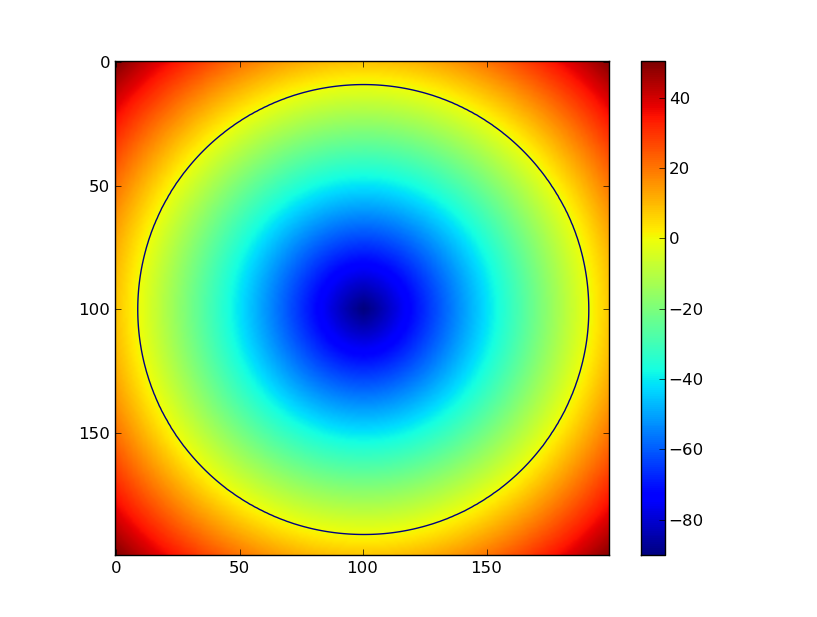
\includegraphics[width=0.50\textwidth]{img/lvl0.png}}
  ~
  \subfloat[$\phi$ and $\Gamma$, some frames
  later.]{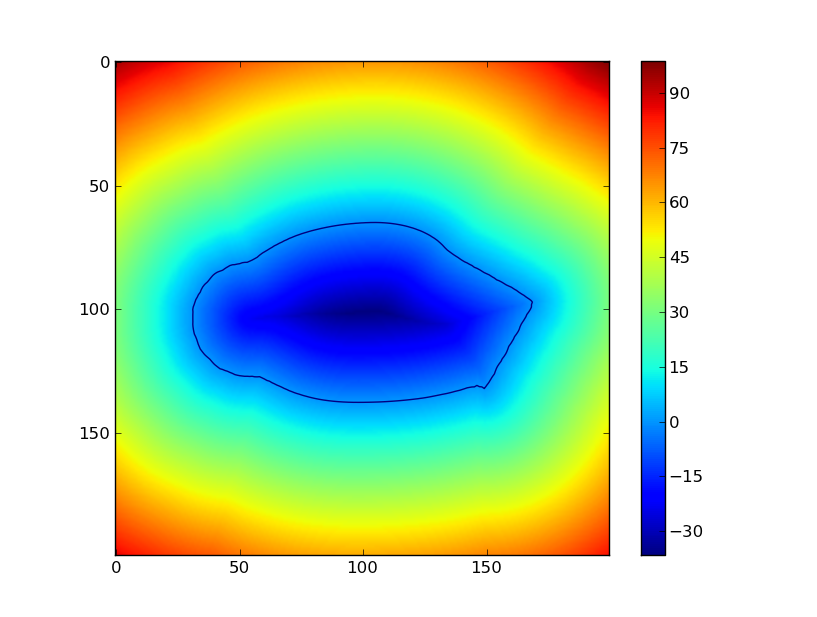
\includegraphics[width=0.50\textwidth]{img/lvl1.png}} \\
  \subfloat[$\phi$ and $\Gamma$ before the topology
  change.]{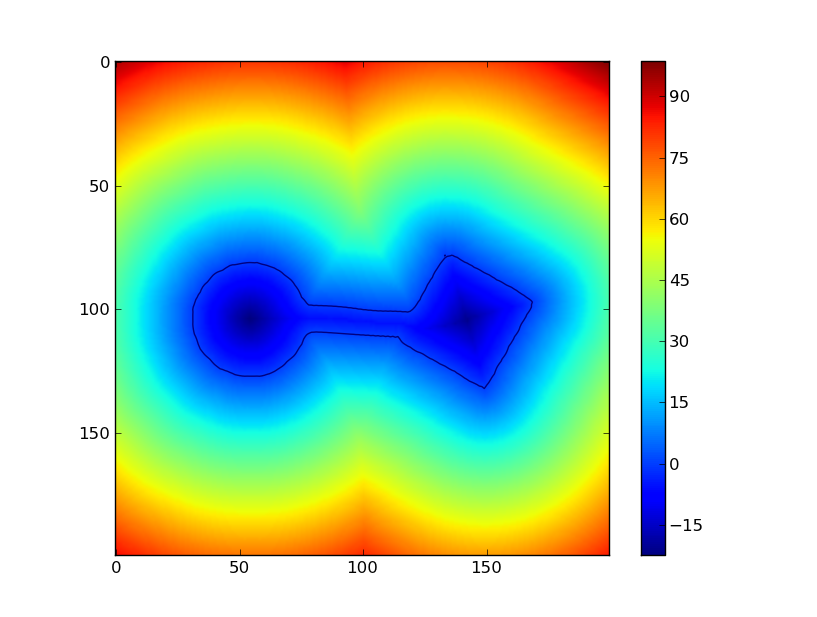
\includegraphics[width=0.50\textwidth]{img/lvl2.png}} ~
  \subfloat[Final stable state of $\phi$ and its level set $\Gamma$.
  ]{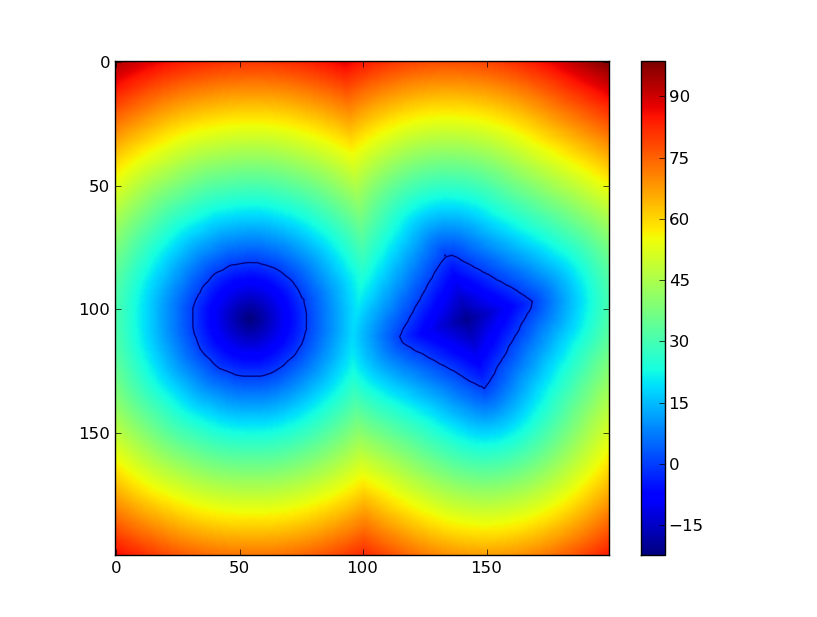
\includegraphics[width=0.50\textwidth]{img/lvl3.png}}
\end{figure}

As stated in section \ref{localmin}, since our implementation is based on
Zhang's force formulation it might sometimes suffer from loss of surface
details. We confirmed this expected behavior using a shape with pronounced
concavities.

\begin{figure}[H]
  \centering
  \subfloat[Shape acting as $S$.]{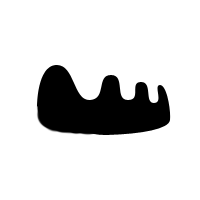
\includegraphics[width=0.50\textwidth]{img/dents.png}} 
  ~
  \subfloat[The level set reaches an unsatisfactory local
  minimum.]{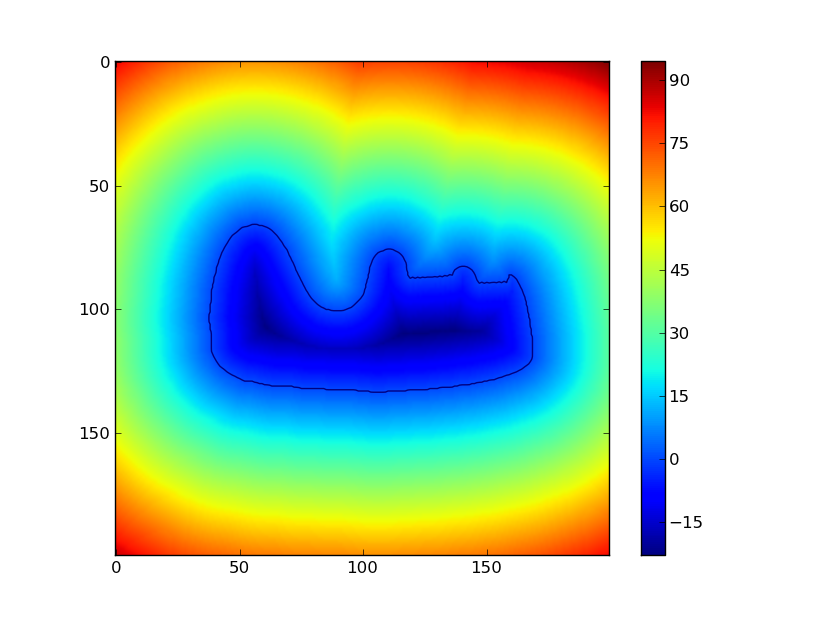
\includegraphics[width=0.50\textwidth]{img/dents_contour.png}}
\end{figure}


\section{Conclusion}

\bibliographystyle{amsplain}
\bibliography{vision}

\end{document}
